%
% meniskus.tex
%
% (c) 2024 Prof Dr Andreas Müller
%
\begin{figure}
\centering
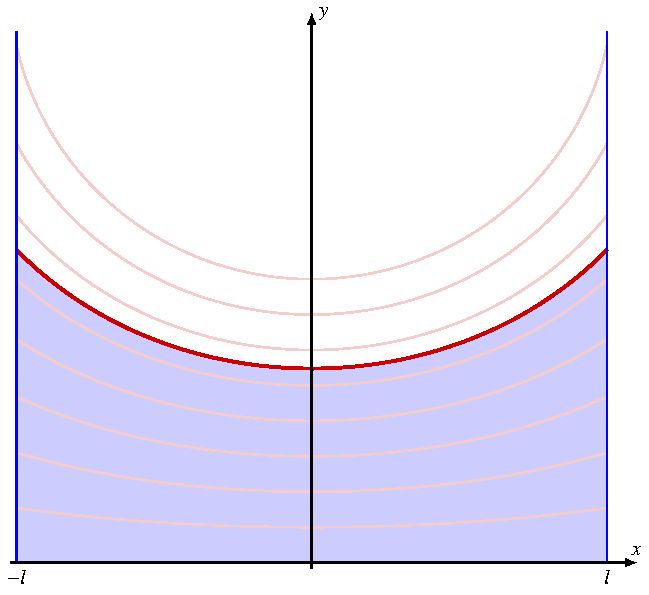
\includegraphics{chapters/050-nebenbedingungen/images/meniskus.pdf}
\caption{Meniskus zwischen zwei parallelen, vertikalen Ebenen
im Abstand $2l$.
Je grössser $\sigma$ ist, desto höher steigt die Flüssigkeitsoberfläche
und desto steiler trifft die Oberfläche auf die Wand.
\label{buch:nebenbedingungen:transversal:fig:meniskus}}
\end{figure}
